% \documentclass{article}
\documentclass[conference,compsoc,10pt]{IEEEtran}

% if you need to pass options to natbib, use, e.g.:
%     \PassOptionsToPackage{numbers, compress}{natbib}
% before loading neurips_2023


% ready for submission
% \usepackage{iclr2024_conference,times}


% to compile a preprint version, e.g., for submission to arXiv, add the
% [preprint] option:
%     \usepackage[preprint]{neurips_2023}


% to compile a camera-ready version, add the [final] option, e.g.:
%     \usepackage[final]{neurips_2023}


% to avoid loading the natbib package, add option nonatbib:
%    \usepackage[nonatbib]{neurips_2023}

\ifCLASSOPTIONcompsoc
  % IEEE Computer Society needs nocompress option
  % requires cite.sty v4.0 or later (November 2003)
  % \usepackage[nocompress]{cite}
  \usepackage[numbers]{natbib}
\else
  % normal IEEE
  % \usepackage{cite}
  \usepackage{natbib}
\fi


\usepackage[utf8]{inputenc} % allow utf-8 input
\usepackage[T1]{fontenc}    % use 8-bit T1 fonts
\usepackage{hyperref}       % hyperlinks
\hypersetup{
    colorlinks,
    linkcolor={red!70!black},
    citecolor={green!70!black},
    urlcolor={blue!80!black}
}
\usepackage{url}            % simple URL typesetting
\usepackage{booktabs}       % professional-quality tables
\usepackage{amsfonts}       % blackboard math symbols
\usepackage{nicefrac}       % compact symbols for 1/2, etc.
\usepackage{microtype}      % microtypography
\usepackage{xcolor}         % colors
\usepackage{enumitem}
\usepackage{amsmath}
\usepackage{amssymb}
\usepackage{mathtools}
\usepackage{tablefootnote}
\usepackage{amsthm}
\usepackage{bbm}
\usepackage{bm}
\usepackage{todonotes}
\usepackage{dblfloatfix}

\usepackage[capitalize]{cleveref}
\usepackage{multirow}
\usepackage{makecell}
\usepackage{wrapfig}
\usepackage{tikz}
\usepackage{xspace}
\usepackage{caption}

\renewcommand{\cellalign}{vh}
\renewcommand{\theadalign}{vh}

\DeclareMathOperator*{\argmax}{arg\,max}
\DeclareMathOperator*{\argmin}{arg\,min}

\newcommand{\hullvolume}[0]{$V_{\text{hull}}$}
\newcommand{\hullarea}[0]{$A_{\text{hull}}$}
\newcommand{\quality}[0]{$Q$}
\newcommand{\efficiency}[0]{$E$}
\newcommand{\robustness}[0]{$R$}

\title{Mark My Words: Analyzing and Evaluating Language Model Watermarks}


% The \author macro works with any number of authors. There are two commands
% used to separate the names and addresses of multiple authors: \And and \AND.
%
% Using \And between authors leaves it to LaTeX to determine where to break the
% lines. Using \AND forces a line break at that point. So, if LaTeX puts 3 of 4
% authors names on the first line, and the last on the second line, try using
% \AND instead of \And before the third author name.

\author{\IEEEauthorblockN{Julien Piet}
\IEEEauthorblockA{\textit{UC Berkeley} }
\and
\IEEEauthorblockN{Chawin Sitawarin}
\IEEEauthorblockA{\textit{UC Berkeley} }
\and
\IEEEauthorblockN{Vivian Fang}
\IEEEauthorblockA{\textit{UC Berkeley} }
\and

\IEEEauthorblockN{Norman Mu}
\IEEEauthorblockA{\textit{UC Berkeley} }
\and
\IEEEauthorblockN{David Wagner}
\IEEEauthorblockA{\textit{UC Berkeley} }
}


\newcommand{\jp}[1]{{\color{green!15!blue}[#1] --Julien}}
\newcommand{\vf}[1]{{\color{violet}[#1] --Vivian}}
\newcommand{\norm}[1]{{\color{green} N: #1}}
\newcommand{\chawin}[1]{{\color{orange} C: #1}}
\newcommand{\dave}[1]{{\color{purple} D: #1}}
\newcommand{\itemlm}{{15pt}}
% \newcommand{\benchmarkname}{{MarkMyWords}}
\newcommand{\benchmarkname}{\textsc{MarkMyWords}}
\newcommand{\scott}{\citet{aaronson_watermarking_2022}}
\newcommand{\mylink}[1]{\url{#1}}
% \newcommand{\mylink}[1]{\texttt{this anonymized link\xspace}}

\begin{document}


\maketitle
\thispagestyle{plain}
\pagestyle{plain}


\begin{abstract}
  The capabilities of large language models have grown significantly in recent years and so too have concerns about their misuse. 
  In this context, the ability to distinguish machine-generated text from human-authored content becomes important. 
  Prior works have proposed numerous schemes to watermark text, which would benefit from a systematic evaluation framework.
  This work focuses on text watermarking techniques --- as opposed to image watermarks --- and proposes \benchmarkname{}, a 
  comprehensive benchmark for them under different tasks 
  as well as practical attacks. We focus on three main metrics: quality, size (e.g. the number of tokens needed to detect a watermark), and tamper-resistance. 
  Current watermarking techniques are good enough to be deployed:~\citet{kirchenbauer_watermark_2023} can 
  watermark Llama2-7B-chat with no perceivable loss in quality, the watermark can be detected with fewer than 100 tokens, and the scheme offers good tamper-resistance to simple attacks. 
  We argue that watermark indistinguishability, a criteria emphasized in some prior works, is too strong a requirement: schemes that slightly modify logit 
  distributions outperform their indistinguishable counterparts with no noticeable loss in generation quality. 
  We publicly release our benchmark (\mylink{https://github.com/wagner-group/MarkMyWords})
\end{abstract}

% !TEX root = ../arxiv.tex

Unsupervised domain adaptation (UDA) is a variant of semi-supervised learning \cite{blum1998combining}, where the available unlabelled data comes from a different distribution than the annotated dataset \cite{Ben-DavidBCP06}.
A case in point is to exploit synthetic data, where annotation is more accessible compared to the costly labelling of real-world images \cite{RichterVRK16,RosSMVL16}.
Along with some success in addressing UDA for semantic segmentation \cite{TsaiHSS0C18,VuJBCP19,0001S20,ZouYKW18}, the developed methods are growing increasingly sophisticated and often combine style transfer networks, adversarial training or network ensembles \cite{KimB20a,LiYV19,TsaiSSC19,Yang_2020_ECCV}.
This increase in model complexity impedes reproducibility, potentially slowing further progress.

In this work, we propose a UDA framework reaching state-of-the-art segmentation accuracy (measured by the Intersection-over-Union, IoU) without incurring substantial training efforts.
Toward this goal, we adopt a simple semi-supervised approach, \emph{self-training} \cite{ChenWB11,lee2013pseudo,ZouYKW18}, used in recent works only in conjunction with adversarial training or network ensembles \cite{ChoiKK19,KimB20a,Mei_2020_ECCV,Wang_2020_ECCV,0001S20,Zheng_2020_IJCV,ZhengY20}.
By contrast, we use self-training \emph{standalone}.
Compared to previous self-training methods \cite{ChenLCCCZAS20,Li_2020_ECCV,subhani2020learning,ZouYKW18,ZouYLKW19}, our approach also sidesteps the inconvenience of multiple training rounds, as they often require expert intervention between consecutive rounds.
We train our model using co-evolving pseudo labels end-to-end without such need.

\begin{figure}[t]%
    \centering
    \def\svgwidth{\linewidth}
    \input{figures/preview/bars.pdf_tex}
    \caption{\textbf{Results preview.} Unlike much recent work that combines multiple training paradigms, such as adversarial training and style transfer, our approach retains the modest single-round training complexity of self-training, yet improves the state of the art for adapting semantic segmentation by a significant margin.}
    \label{fig:preview}
\end{figure}

Our method leverages the ubiquitous \emph{data augmentation} techniques from fully supervised learning \cite{deeplabv3plus2018,ZhaoSQWJ17}: photometric jitter, flipping and multi-scale cropping.
We enforce \emph{consistency} of the semantic maps produced by the model across these image perturbations.
The following assumption formalises the key premise:

\myparagraph{Assumption 1.}
Let $f: \mathcal{I} \rightarrow \mathcal{M}$ represent a pixelwise mapping from images $\mathcal{I}$ to semantic output $\mathcal{M}$.
Denote $\rho_{\bm{\epsilon}}: \mathcal{I} \rightarrow \mathcal{I}$ a photometric image transform and, similarly, $\tau_{\bm{\epsilon}'}: \mathcal{I} \rightarrow \mathcal{I}$ a spatial similarity transformation, where $\bm{\epsilon},\bm{\epsilon}'\sim p(\cdot)$ are control variables following some pre-defined density (\eg, $p \equiv \mathcal{N}(0, 1)$).
Then, for any image $I \in \mathcal{I}$, $f$ is \emph{invariant} under $\rho_{\bm{\epsilon}}$ and \emph{equivariant} under $\tau_{\bm{\epsilon}'}$, \ie~$f(\rho_{\bm{\epsilon}}(I)) = f(I)$ and $f(\tau_{\bm{\epsilon}'}(I)) = \tau_{\bm{\epsilon}'}(f(I))$.

\smallskip
\noindent Next, we introduce a training framework using a \emph{momentum network} -- a slowly advancing copy of the original model.
The momentum network provides stable, yet recent targets for model updates, as opposed to the fixed supervision in model distillation \cite{Chen0G18,Zheng_2020_IJCV,ZhengY20}.
We also re-visit the problem of long-tail recognition in the context of generating pseudo labels for self-supervision.
In particular, we maintain an \emph{exponentially moving class prior} used to discount the confidence thresholds for those classes with few samples and increase their relative contribution to the training loss.
Our framework is simple to train, adds moderate computational overhead compared to a fully supervised setup, yet sets a new state of the art on established benchmarks (\cf \cref{fig:preview}).

\section{Background and Motivation}

\subsection{IBM Streams}

IBM Streams is a general-purpose, distributed stream processing system. It
allows users to develop, deploy and manage long-running streaming applications
which require high-throughput and low-latency online processing.

The IBM Streams platform grew out of the research work on the Stream Processing
Core~\cite{spc-2006}.  While the platform has changed significantly since then,
that work established the general architecture that Streams still follows today:
job, resource and graph topology management in centralized services; processing
elements (PEs) which contain user code, distributed across all hosts,
communicating over typed input and output ports; brokers publish-subscribe
communication between jobs; and host controllers on each host which
launch PEs on behalf of the platform.

The modern Streams platform approaches general-purpose cluster management, as
shown in Figure~\ref{fig:streams_v4_v6}. The responsibilities of the platform
services include all job and PE life cycle management; domain name resolution
between the PEs; all metrics collection and reporting; host and resource
management; authentication and authorization; and all log collection. The
platform relies on ZooKeeper~\cite{zookeeper} for consistent, durable metadata
storage which it uses for fault tolerance.

Developers write Streams applications in SPL~\cite{spl-2017} which is a
programming language that presents streams, operators and tuples as
abstractions. Operators continuously consume and produce tuples over streams.
SPL allows programmers to write custom logic in their operators, and to invoke
operators from existing toolkits. Compiled SPL applications become archives that
contain: shared libraries for the operators; graph topology metadata which tells
both the platform and the SPL runtime how to connect those operators; and
external dependencies. At runtime, PEs contain one or more operators. Operators
inside of the same PE communicate through function calls or queues. Operators
that run in different PEs communicate over TCP connections that the PEs
establish at startup. PEs learn what operators they contain, and how to connect
to operators in other PEs, at startup from the graph topology metadata provided
by the platform.

We use ``legacy Streams'' to refer to the IBM Streams version 4 family. The
version 5 family is for Kubernetes, but is not cloud native. It uses the
lift-and-shift approach and creates a platform-within-a-platform: it deploys a
containerized version of the legacy Streams platform within Kubernetes.

\subsection{Kubernetes}

Borg~\cite{borg-2015} is a cluster management platform used internally at Google
to schedule, maintain and monitor the applications their internal infrastructure
and external applications depend on. Kubernetes~\cite{kube} is the open-source
successor to Borg that is an industry standard cloud orchestration platform.

From a user's perspective, Kubernetes abstracts running a distributed
application on a cluster of machines. Users package their applications into
containers and deploy those containers to Kubernetes, which runs those
containers in \emph{pods}. Kubernetes handles all life cycle management of pods,
including scheduling, restarting and migration in case of failures.

Internally, Kubernetes tracks all entities as \emph{objects}~\cite{kubeobjects}.
All objects have a name and a specification that describes its desired state.
Kubernetes stores objects in etcd~\cite{etcd}, making them persistent,
highly-available and reliably accessible across the cluster. Objects are exposed
to users through \emph{resources}. All resources can have
\emph{controllers}~\cite{kubecontrollers}, which react to changes in resources.
For example, when a user changes the number of replicas in a
\code{ReplicaSet}, it is the \code{ReplicaSet} controller which makes sure the
desired number of pods are running. Users can extend Kubernetes through
\emph{custom resource definitions} (CRDs)~\cite{kubecrd}. CRDs can contain
arbitrary content, and controllers for a CRD can take any kind of action.

Architecturally, a Kubernetes cluster consists of nodes. Each node runs a
\emph{kubelet} which receives pod creation requests and makes sure that the
requisite containers are running on that node. Nodes also run a
\emph{kube-proxy} which maintains the network rules for that node on behalf of
the pods. The \emph{kube-api-server} is the central point of contact: it
receives API requests, stores objects in etcd, asks the scheduler to schedule
pods, and talks to the kubelets and kube-proxies on each node. Finally,
\emph{namespaces} logically partition the cluster. Objects which should not know
about each other live in separate namespaces, which allows them to share the
same physical infrastructure without interference.

\subsection{Motivation}
\label{sec:motivation}

Systems like Kubernetes are commonly called ``container orchestration''
platforms. We find that characterization reductive to the point of being
misleading; no one would describe operating systems as ``binary executable
orchestration.'' We adopt the idea from Verma et al.~\cite{borg-2015} that
systems like Kubernetes are ``the kernel of a distributed system.'' Through CRDs
and their controllers, Kubernetes provides state-as-a-service in a distributed
system. Architectures like the one we propose are the result of taking that view 
seriously.

The Streams legacy platform has obvious parallels to the Kubernetes
architecture, and that is not a coincidence: they solve similar problems.
Both are designed to abstract running arbitrary user-code across a distributed
system.  We suspect that Streams is not unique, and that there are many
non-trivial platforms which have to provide similar levels of cluster
management.  The benefits to being cloud native and offloading the platform
to an existing cloud management system are: 
\begin{itemize}
    \item Significantly less platform code.
    \item Better scheduling and resource management, as all services on the cluster are 
        scheduled by one platform.
    \item Easier service integration.
    \item Standardized management, logging and metrics.
\end{itemize}
The rest of this paper presents the design of replacing the legacy Streams 
platform with Kubernetes itself.


\section{Assumptions for security}
\label{sec:attacks}

The security of a quantum cryptographic protocol relies on assumptions about the physics of the devices that are employed to implement the protocol.  In this section, we discuss these assumptions. For concreteness, we focus on the case of QKD, for which we describe the full set of assumptions in \secref{sec:attacks:assumptionlist}.  We then explain why these assumptions are needed and to what extent they are justified in \secref{sec:attacks:necessity}. Experimental work in QKD has shown however that the assumptions are often very difficult to meet, and are actually not met in many cases. This fact can be exploited by quantum hacking attacks, which are described in \ref{sec:attacks:hacking}. Finally, in Section~\ref{sec:attacks:countermeasures}, we discuss countermeasures against these attacks. 

\subsection{Standard assumptions for QKD} \label{sec:attacks:assumptionlist}

The security of QKD protocols usually relies on the following assumptions.

\begin{enumerate}
  \item \label{item_qm} All devices used by Alice and Bob, as well as the communication channels connecting them, are correctly and completely\footnote{The completeness of quantum theory can be derived from their correctness;  see \secref{sec:completeness}.} described by quantum theory.
    \item \label{item_res} The channel that Alice and Bob use to exchange classical messages is authentic, i.e., it is impossible for an adversary to modify messages or insert new ones. 
  \item \label{item_conv} The devices that Alice and Bob use locally to execute the steps of the protocol, e.g., for preparing and measuring quantum systems, do exactly what they are instructed to do.
\end{enumerate}

As already indicated earlier, due to the lack of proof techniques, additional assumptions had been introduced in the past. A prominent example is the \emph{i.i.d.}\ assumption, which demands that the quantum channel connecting Alice and Bob be described by a sequence of identical and independently distributed maps. Physically, this means that an adversary's interception strategy is such that each signal sent from Alice to Bob is modified in the same manner and independently of the other signals. Security under the i.i.d.\ assumption is called security against \emph{collective attacks}~\cite[see also \secref{sec:qkd.other.models}]{BM97b,BBBvdGM02}. Another assumption, which  usually comes on top of the i.i.d.\ assumption, is that Eve only stores classical data, which she obtains by individually measuring the pieces of information she gained from each signal sent from Alice to Bob. Since it is difficult to argue why an adversary should be restricted in that particular way, the corresponding security guarantee is rather weak. It is usually referred to as security against \emph{individual attacks}~\cite[see \secref{sec:qkd.other.models}]{Fuchsetal1997,Lutkenhaus2000}. 

Most modern security proofs do however not require such additional assumptions, i.e., they are based entirely on Assumptions~\ref{item_qm}--\ref{item_conv} above. This means, in particular, that the quantum channel connecting Alice and Bob can be arbitrary, and may even be entirely controlled by Eve. In this case, one talks about security against \emph{general attacks}, \emph{coherent attacks}, or \emph{joint attacks}. Sometimes the term  \emph{unconditional security} appeared in the literature~\cite{SBCDLP09}, but it is important to keep in mind that the assumptions listed above are still necessary.

\subsection{Necessity and justification of assumptions} \label{sec:attacks:necessity}

Assumption~\ref{item_qm} is often implicit, for it is a prerequisite to even describe the cryptographic scheme. It justifies the use of the formalism of quantum theory to model the different systems, such as the communication channel, including any possible attacks on them. The assumption thus captures the main idea behind quantum cryptography, namely that an adversary is limited by the laws of quantum theory.  The other two assumptions ensure that the experimental implementation follows the theoretical prescription that enters the security definition (Definition~\ref{def:security}), namely the description of the protocol $\pi_{AB}$ and the used resources. In particular, Assumption~\ref{item_res} guarantees that the resources shared between Alice and Bob fulfil the theoretical specifications~$\aR$, which in the case of QKD includes the classical authentic communication channel. Assumption~\ref{item_conv} guarantees that the steps prescribed by the protocol~$\pi_{A B}$ are correctly executed.

Assumption~\ref{item_qm} is widely accepted \--- and proving it wrong would represent a major breakthrough in physics. Nevertheless, it has been shown that there exist QKD protocols that only rely on the weaker assumption of \emph{no-signalling}~\cite{BHK05}.  

Assumption~\ref{item_res} demands that an authentic communication channel is set up between Alice and Bob. There exist information-theoretically secure protocols that achieve this, provided that Alice and Bob share a weak secret key~\cite[see also \secref{sec:smt.auth}]{RW03,DW09,ACLV19}.  Assumption~\ref{item_res} can thus be met by the use of such authentication protocols (see also~\secref{sec:intro} as well as standard textbooks on classical cryptography)

Although Assumption~\ref{item_conv} sounds rather natural, and is in fact required for almost any cryptographic scheme, including any classical one, it is rather challenging to meet.  Numerous quantum hacking experiments, which have been conducted over the past few years, have shown that many implementations of QKD failed to satisfy this assumption. To illustrate this problem, we describe selected examples of such attacks in the following subsection.

\subsection{Quantum hacking attacks} \label{sec:attacks:hacking}          

We start with the \emph{photon number splitting attack}~\cite{Brassardetal2000}, which targets optical implementations of QKD that use individual photons as quantum information carriers. Suppose, for concreteness, that Alice and Bob implement the BB84 protocol~\cite{BB84} by encoding the qubits into the polarisation degree of freedom of individual photons. Specifically, Alice may use a single-photon source that emits photons with a polarisation that she can choose. The BB84 protocol\footnote{This protocol is explained in more detail in \secref{sec:securityproofs}, where a security proof is also sketched.} requires her to send in each round at random a state from one orthonormal basis, say $\{\ket{h}, \ket{v}\}$, where $\ket{h}$ may be realised by a horizontally polarised photon and $\ket{v}$ by a vertically polarised one, or from a complementary basis $\{\ket{d^+}, \ket{d^-}\}$, where $\ket{d^+} = \smash{\frac{1}{\sqrt{2}}} (\ket{h} + \ket{v})$ and $\ket{d^-} = \smash{\frac{1}{\sqrt{2}}} (\ket{h} - \ket{v})$. It may now happen that, in an experimental implementation, the source sometimes accidentally emits two photons at once, which then carry the same polarisation. The states emitted in the four cases are thus $\ket{h} \otimes \ket{h}$, $\ket{v} \otimes \ket{v}$, $\ket{d^+} \otimes \ket{d^+}$, and $\ket{d^-} \otimes \ket{d^-}$.

Before describing the actual attack, we first give a simple information-theoretic argument for why this is problematic. Note first that one single photon carries no information about the choice of the basis made by Alice. Indeed, for either of the basis choices, the density operator describing the photon is maximally mixed, i.e., $\frac{1}{2} \proj{h} + \frac{1}{2} \proj{v} = \frac{1}{2} \proj{d^+} + \frac{1}{2} \proj{d^-} =  \frac{1}{2} \mathbf{1}$. This is however no longer the case for a pulse consisting of two photons, i.e., 
\begin{align}
  \frac{1}{2} \proj{h}^{\otimes 2} + \frac{1}{2} \proj{v}^{\otimes 2} \neq \frac{1}{2} \proj{d^+}^{\otimes 2} + \frac{1}{2} \proj{d^-}^{\otimes 2} \ .
\end{align}
Hence, if the source accidentally emits two equally polarised photons instead of one, it reveals information about Alice's basis choice, which it shouldn't. 

It is therefore not surprising that such two-photon pulses can be exploited by an adversary to attack the system. Eve, who intercepts the channel, may split the two-photon pulse into two, keep one of the photons and send the other one to Bob. The latter thus receives photons in exactly the way prescribed by the protocol, and hence does not notice the interception. Eve, meanwhile, may measure the photons she captured. In principle, if Eve had quantum memory, she could even wait with the measurement until Alice announces the basis choice to Bob, and hence always gain full information about the polarisation state that Alice prepared. 

While the photon number splitting attack exploits an imperfection of the sender (namely that it sometimes emits two identically polarised photons instead of one), many quantum attacks are targeted towards the receiver. An example is the \emph{time-shift attack}~\cite{Makarovetal2006,qi2007time,Zhaoetal2008}, which exploits inaccuracies of the photon detectors. In order to avoid dark counts, the photon detectors are often set up such that they only count photons that arrive within a small time window around the time when a signal is expected to arrive. Furthermore, Bob's receiver device may consist of more than one detector, e.g., one for each possible polarisation state. The time windows of the different detectors are then never perfectly synchronised. This means that there are times at which the receiver is more sensitive to signals with respect to one polarisation than another. Eve may therefore, by appropriately delaying the signals sent from Alice and Bob, bias the detected signals towards one or the other polarisation, and thus gain information about what Bob measures. While this information may be partial, it can, together with the error correction information that is available to Eve, be sufficient to infer the final key. 

Another attack that is targeted towards the receiver is the \emph{detector blinding attack} ~\cite{Makarov2009,WKRFNW11,LWWESM10,GLLSKM11}, where the adversary tries to control the detectors by illuminating them with bright laser light.  In a QKD implementation that uses the encoding of information into the polarisation of individual photons, the detectors are usually configured such they can optimally detect single photon pulses. That is, they should click whenever the incoming pulse contains a photon, and not click if the pulse is empty.  However, the behaviour of such detectors may be rather different in a regime where the incoming pulses contain many photons. For example, it could be that they always click when they are exposed to bright light with a particular intensity, and they may never click for another intensity. Hence, by sending in light with appropriately chosen polarisation and intensity, Eve may gain immediate control over the clicks of Bob's detector. To exploit this for an attack, Eve may mimic Bob's receiver, i.e., intercept the photons sent from Alice and measure them in a randomly chosen basis, as Bob would do. She then sends bright light to Bob to ensure that he obtains the same detector clicks as if he had directly obtained Alice's photons. This works particularly well for implementations that use a \emph{passive basis choice}, i.e., where Bob's measurement basis is not  provided as an input, but rather made by the detection device itself. In this case, an adversary can essentially remote-control Bob and thus get hold of the entire key. 

Yet another hacking strategy are \emph{Trojan-horse attacks}~\cite{Vakhitov2001,GisinFaselKraus2006}. Here the idea is to send a bright laser pulse via the optical fibre into Alice or Bob's component to extract information about its internal settings. Depending on the sender and receiver hardware which is used, measuring the reflection of the pulse can allow Eve, for instance, to determine the basis choices made by Alice and Bob.

In some optical implementations of QKD, e.g., in the \emph{plug-and-play}~\cite{Muller97} or the \emph{circular-type}~\cite{Nishioka2002} system, Alice does not have a photon source but instead encodes information by modulating an incoming signal from Bob before sending it back to him. The signal thus travels twice in opposite directions through the same optical links, which helps reducing fluctuations due to birefringence  and environmental noise. The two-fold use of the (insecure) channel however opens additional possibilities of attacks~\cite{GisinFaselKraus2006}. A prominent example is the \emph{phase-remapping attack}~\cite{FQTL07,XQL10}. It exploits the fact that the modulator used by Alice to encode information into the signal coming from Bob acts on that signal during a particular time interval. In the attack, the adversary slightly advances or delays the signal on its way from Bob to Alice, so that it no longer lies fully within that time interval. The modulation by Alice will then be incomplete, which means that the encoding of the information in the signal differs from what is foreseen by the protocol. This can in turn be exploited by Eve in an intercept-and-resend attack on the signal returned from Alice to Bob. 


\subsection{Countermeasures against quantum hacking} \label{sec:attacks:countermeasures}

The attacks described here have in common that they all exploit a breakdown of Assumption~\ref{item_conv}. Specifically, in the case of the photon-splitting attack, the device used by Alice sends out more information than it is supposed to. In the case of the time-shift attack, it is Bob's measurement device  whose measurement operators are not constant over time and can even be partially controlled by Eve. Finally, in the case of the detector blinding attack on systems with passive basis choice, Eve even takes over control of the randomness used to choose the basis.

A seemingly obvious countermeasure to prevent such attacks is to manufacture sources and detectors that meet the theoretical specifications. That is, one would need a perfect single-photon source, as well as detectors that are perfectly efficient and only measure photon pulses in a specified parameter regime. Such requirements are however unrealistic --- the devices used in experiments will always, at least slightly, deviate from these specifications. 

The other possibility is to develop cryptographic protocols and  security proofs that tolerate imperfections of the devices~\cite{GLLP04}.  This has been done in particular for the attacks described above. To prevent photon number splitting attacks, an efficient countermeasure is the \emph{decoy-state} method~\cite{Hwang2003,Wang2005,Loetal2005}. The idea here is that Alice sometimes deliberately sends multi-photon pulses. Alice and Bob can  then check statistically whether an adversary captured them. Another possibility is to use protocols where Alice's encoding of information has the property that, even when one photon is extracted from a pulse, the information about what Alice sent is still partial~\cite{SARG,TamakiLo,SYK14}. In the case of time-shift attacks, it is sufficient to characterise the maximum bias in the detector efficiencies that can be introduced and account for it in the security proofs. Finally, for the detector blinding attacks, a possible countermeasure is to add tests to the protocol, such as a monitoring of the photocurrent, in order to detect those~\cite{Yuanetal2010}.  

The main problem with such countermeasures is however that the space of possible imperfections is hard to characterise. The above are just a few examples of attacks, and many others have been proposed, and sometimes even demonstrated to work successfully in experiments. For example, an adversary may exploit imperfections in the randomness that Alice and Bob use for choosing their measurement basis. To prevent such attacks, one may again extend the protocols such that they can tolerate imperfect randomness (see \secref{sec:alternative.randomness}). 



The last decade has thus seen an arms race between designers and attackers of quantum cryptographic schemes. A possible way out of this unsatisfactory situation is \emph{device-independent cryptography}. Here the idea is to replace Assumption~\ref{item_conv} by something much weaker. Namely, one requires that the devices used by Alice and Bob do not unintentionally send information out to an adversary, and that the classical processing of information done by Alice and Bob is correct. Crucially, however,  one does no longer demand that the sources and detectors used by Alice and Bob work according to their specifications. The way this can work is explained in \secref{sec:alternative.di}. 

%%% Local Variables:
%%% TeX-master: "main.tex"
%%% End:

\subsection{Evaluation metrics}
\label{sup:eval}
Performance was evaluated using precision@$k$ and nDCG@$k$ metrics. Performance was also evaluated using propensity scored metrics, namely propensity scored precision@$k$ and nDCG@$k$ (with $k$ = 1, 3 and 5) for extreme classification. The propensity scoring model and values available on The Extreme Classification Repository~\citep{XMLRepo} were used for the publicly available datasets. For the proprietary datasets, the method outlined in \cite{Jain16} was used. For a predicted score vector $\hat{\mathbf{y}} \in R^L$ and ground truth label vector $\mathbf{y} \in \{0, 1\}^L$, the metrics are defined below. In the following, $p_l$ is propensity score of the label $l$ as proposed in~\citep{Jain16}.
\begin{flalign}
P@k&= \frac{1}{k} {\sum_{l \in rank_k(\hat{\mathbf{y}})}} y_l &
PSP@k&= \frac{1}{k} {\sum_{l \in rank_k(\hat{\mathbf{y}})}} \frac{y_l}{p_l} & \nonumber\\
DCG@k&= \frac{1}{k} {\sum_{l \in rank_k(\hat{\mathbf{y}})}} \frac{y_l}{\log(l+1)} \nonumber
& PSDCG@k&= \frac{1}{k} {\sum_{l \in rank_k(\hat{\mathbf{y}})}} \frac{y_l}{p_l \log(l+1)} & \nonumber\\
nDCG@k&= \frac{DCG@k}{\sum_{l=1}^{\min(k, ||\mathbf{y}||_0)} \frac{1}{\log(l +1) }} \nonumber
 &
PSnDCG@k&= \frac{PSDCG@k}{\sum_{l=1}^{k} \frac{1}{\log l +1 }} &\nonumber,
\end{flalign}

\section{\benchmarkname{}}
\label{sec:experiments}

% DONE: I think it might help to have a name for the benchmark,
% and to use that throughout the paper.  Then others who use the
% benchmark can refer to it by that name.

% We can call it MarkMyWords

% Our benchmark measures a watermark's quality, efficiency, and tamper-resistance in various contexts.
%
We now present \benchmarkname{}, our benchmark for evaluating watermarking schemes.

\subsection{Text Generation Tasks}

%Our benchmark relies on three tasks, all intended to generate long-form text, while also representing real scenarios in which one would wish to watermark the model outputs.
%

\benchmarkname{} uses three text generation tasks.
There were chosen to generate long text, in order to ensure enough tokens to watermark most outputs and get a good size estimate,
and to represent realistic scenarios in which watermarking would be useful.
We watermark the outputs of each task and measure quality, watermark size, and tamper-resistance on these outputs.
\cref{tab:bench-prompts} shows the prompt for each task.

\smallskip\noindent\textbf{(1) Book reports.}
%
Our first task instructs the model to generate book reports for a predefined list of 100 well-known books.
%
This represents a realistic use case of a watermark in an education context where instructors might wish to verify if students have used a language 
model to complete their homework assignment.
%
% Our prompt format is ``Write a book report about X, written by Y.'',
% where X is a book title and Y is the book's author. 

\smallskip\noindent\textbf{(2) Story generation.}
%
We ask the model to generate a short story, with a specific tone (e.g., funny, sad, suspenseful), on a particular topic (e.g., ``three strangers that win a getaway vacation together'').
%
We use 100 combinations of topics and tones.
%
In this case, detecting watermarks in creative content is a way to trace the authorship of a 
piece of text.
% Our prompt is ``Write a X story about Y.'', where X is the tone, and Y is the topic.

\smallskip\noindent\textbf{(3) Fake news.}
%
Our last task asks the model to generate a news story about two prominent political figures meeting at an event.
%
In total, we have a list of 100 unique combinations of political figures and locations.
%
Detecting watermarks in short news articles or headlines could be useful for fighting against automated fake news bots on social media.
%
% Our prompt is ``Write a news article about X's visit to Y in Z.'', where X and Y are two political figures, and Z is a location.

\subsection{Benchmark Implementation}

We implemented the \benchmarkname{} benchmark in Python using the \texttt{transformers} library~\citep{wolf_transformers_2020} to implement models and watermarks.
%
In general, the run times of the watermarked models are comparable to those of base models.
%
We rely on the 7B-parameter version of Llama-2 chat both for generation and rating.
%
We chose this model for its high quality and because its output distribution, like other modern models, has low entropy.
We've noticed newer language models are more certain of their next-token predections, i.e., have lower entropy in their output distribution,
which makes watermarking more difficult. Thus, using a low-entropy model makes for a more realistic 
evaluation of a watermark scheme's performance. 
%
This version of the Llama-2 model is known for often refusing to generate content---we 
altered the system prompt to avoid this issue, especially for the fake news task.

Our benchmark generates a total of 300 outputs from the language model.
%
We only attack a third of these (the first third of each task),
as running robustness tests on all 300 would make the benchmark too slow.
%
The maximum number of generated tokens per prompt is 1024.
%
On a A5000 GPU, the benchmark completes in 30 minutes to an hour. 

%Users can choose whether to sample a new secret watermarking key for each generation or not.
%
%We enable this in our experiments, but practitioners can deactivate it in order to evaluate a model's performance for a specific secret key, for instance when evaluating a public scheme.

Our code for the \benchmarkname{} benchmark has been made public.\footnote{\mylink{https://github.com/wagner-group/MarkMyWords}}
%
It is easily updated to support new watermarking schemes or new language models.
%Anyone can run it, either to compare new watermarking schemes to the ones presented in the paper, or to find the best hyper-parameter 
%selection for another language model. 
%
We hope that future proposals of watermark schemes will include an evaluation with this benchmark.

\smallskip\noindent\textbf{Efficiency.}
%
We have developed custom implementations directly in CUDA of some of the watermarking schemes, to speed up computation.
\begin{itemize}[leftmargin=\itemlm,nosep]
    \item \textbf{Hash function.} The exponential sampling scheme relies on computing the hash of many elements. Our CUDA implementation allows this to be done in parallel.
    \item \textbf{Edit distance.} The edit distance is computed with every possible key offset; our code implements this in parallel.
\end{itemize}
% Additionally, for empirical verification of edit scores, since we use a $t$-test~\cite{kuditipudi_robust_2023}, we need to compute test statistic 100 times under the null hypothesis to derive an empirical $p$-value.
% %
% This is done by replacing the randomness used at generation time by fresh random 
% values.
% Doing so for each detection is inefficient.
% %
% Instead, for edit scores, we pre-compute the test statistic under the null hypothesis 200 times and then sample 100 random values of this statistic every time we want to verify a watermark.
% \chawin{I'm a bit confused by this part.}
% %
% This means we only need to run the expensive computation once.
% %
% Empirically, we did not see a change in detection accuracy when doing so. 

%!TEX ROOT = ../../centralized_vs_distributed.tex

\section{{\titlecap{the centralized-distributed trade-off}}}\label{sec:numerical-results}

\revision{In the previous sections we formulated the optimal control problem for a given controller architecture
(\ie the number of links) parametrized by $ n $
and showed how to compute minimum-variance objective function and the corresponding constraints.
In this section, we present our main result:
%\red{for a ring topology with multiple options for the parameter $ n $},
we solve the optimal control problem for each $ n $ and compare the best achievable closed-loop performance with different control architectures.\footnote{
\revision{Recall that small (large) values of $ n $ mean sparse (dense) architectures.}}
For delays that increase linearly with $n$,
\ie $ f(n) \propto n $, 
we demonstrate that distributed controllers with} {few communication links outperform controllers with larger number of communication links.}

\textcolor{subsectioncolor}{Figure~\ref{fig:cont-time-single-int-opt-var}} shows the steady-state variances
obtained with single-integrator dynamics~\eqref{eq:cont-time-single-int-variance-minimization}
%where we compare the standard multi-parameter design 
%with a simplified version \tcb{that utilizes spatially-constant feedback gains
and the quadratic approximation~\eqref{eq:quadratic-approximation} for \revision{ring topology}
with $ N = 50 $ nodes. % and $ n\in\{1,\dots,10\} $.
%with $ N = 50 $, $ f(n) = n $ and $ \tau_{\textit{min}} = 0.1 $.
%\autoref{fig:cont-time-single-int-err} shows the relative error, defined as
%\begin{equation}\label{eq:relative-error}
%	e \doteq \dfrac{\optvarx-\optvar}{\optvar}
%\end{equation}
%where $ \optvar $ and $ \optvarx $ denote the the optimal and sub-optimal scalar variances, respectively.
%The performance gap is small
%and becomes negligible for large $ n $.
{The best performance is achieved for a sparse architecture with  $ n = 2 $ 
in which each agent communicates with the two closest pairs of neighboring nodes. 
This should be compared and contrasted to nearest-neighbor and all-to-all 
communication topologies which induce higher closed-loop variances. 
Thus, 
the advantage of introducing additional communication links diminishes 
beyond}
{a certain threshold because of communication delays.}

%For a linear increase in the delay,
\textcolor{subsectioncolor}{Figure~\ref{fig:cont-time-double-int-opt-var}} shows that the use of approximation~\eqref{eq:cont-time-double-int-min-var-simplified} with $ \tilde{\gvel}^* = 70 $
identifies nearest-neighbor information exchange as the {near-optimal} architecture for a double-integrator model
with ring topology. 
This can be explained by noting that the variance of the process noise $ n(t) $
in the reduced model~\eqref{eq:x-dynamics-1st-order-approximation}
is proportional to $ \nicefrac{1}{\gvel} $ and thereby to $ \taun $,
according to~\eqref{eq:substitutions-4-normalization},
making the variance scale with the delay.

%\mjmargin{i feel that we need to comment about different results that we obtained for CT and DT double-intergrator dynamics (monotonic deterioration of performance for the former and oscillations for the latter)}
\revision{\textcolor{subsectioncolor}{Figures~\ref{fig:disc-time-single-int-opt-var}--\ref{fig:disc-time-double-int-opt-var}}
show the results obtained by solving the optimal control problem for discrete-time dynamics.
%which exhibit similar trade-offs.
The oscillations about the minimum in~\autoref{fig:disc-time-double-int-opt-var}
are compatible with the investigated \tradeoff~\eqref{eq:trade-off}:
in general, 
the sum of two monotone functions does not have a unique local minimum.
Details about discrete-time systems are deferred to~\autoref{sec:disc-time}.
Interestingly,
double integrators with continuous- (\autoref{fig:cont-time-double-int-opt-var}) ad discrete-time (\autoref{fig:disc-time-double-int-opt-var}) dynamics
exhibits very different trade-off curves,
whereby performance monotonically deteriorates for the former and oscillates for the latter.
While a clear interpretation is difficult because there is no explicit expression of the variance as a function of $ n $,
one possible explanation might be the first-order approximation used to compute gains in the continuous-time case.
%which reinforce our thesis exposed in~\autoref{sec:contribution}.

%\begin{figure}
%	\centering
%	\includegraphics[width=.6\linewidth]{cont-time-double-int-opt-var-n}
%	\caption{Steady-state scalar variance for continuous-time double integrators with $ \taun = 0.1n $.
%		Here, the \tradeoff is optimized by nearest-neighbor interaction.
%	}
%	\label{fig:cont-time-double-int-opt-var-lin}
%\end{figure}
}

\begin{figure}
	\centering
	\begin{minipage}[l]{.5\linewidth}
		\centering
		\includegraphics[width=\linewidth]{random-graph}
	\end{minipage}%
	\begin{minipage}[r]{.5\linewidth}
		\centering
		\includegraphics[width=\linewidth]{disc-time-single-int-random-graph-opt-var}
	\end{minipage}
	\caption{Network topology and its optimal {closed-loop} variance.}
	\label{fig:general-graph}
\end{figure}

Finally,
\autoref{fig:general-graph} shows the optimization results for a random graph topology with discrete-time single integrator agents. % with a linear increase in the delay, $ \taun = n $.
Here, $ n $ denotes the number of communication hops in the ``original" network, shown in~\autoref{fig:general-graph}:
as $ n $ increases, each agent can first communicate with its nearest neighbors,
then with its neighbors' neighbors, and so on. For a control architecture that utilizes different feedback gains for each communication link
	(\ie we only require $ K = K^\top $) we demonstrate that, in this case, two communication hops provide optimal closed-loop performance. % of the system.}

Additional computational experiments performed with different rates $ f(\cdot) $ show that the optimal number of links increases for slower rates: 
for example, 
the optimal number of links is larger for $ f(n) = \sqrt{n} $ than for $ f(n) = n $. 
\revision{These results are not reported because of space limitations.}
\section{Designing a Watermark}
\label{sec:taxonomy}

After the quick overview of watermarking schemes in \cref{sec:background}, we now provide more details 
about the watermarking design space. We created a unifying taxonomy under which all previous schemes 
can be expressed. We first discuss the requirements then the building blocks of a text watermark. 
%
%We provide a modular implementation of all schemes, so any of the building blocks can be combined.
%
\cref{fig:design-figure} summarizes the current design space.

\subsection{Requirements}

A useful watermarking scheme must detect watermarked texts, without falsely flagging human-generated text and without impairing the original model's performance.
%
More precisely, we want watermarks to have the following properties.
% \begin{itemize}[leftmargin=\itemlm,itemsep=2pt]
\begin{enumerate}[leftmargin=\itemlm,itemsep=2pt]
    \item \textbf{High Recall}. $\Pr[\mathcal{V}_k(T) = \texttt{True}]$ is large if $T$ is a watermarked text generated using the marking procedure $\mathcal{W}$ and secret key $k$.
    %
    \item \textbf{High Precision}. For a random key $k$, $\Pr[\mathcal{V}_k(\Tilde{T}) = \texttt{False}]$ is large if $\Tilde{T}$ is a human-generated (\emph{non-watermarked}) text.
    %
    \item \textbf{Quality}. The watermarked model should perform similarly to the original model. 
    It should be useful for the same tasks and generate similar quality text.
    %
    \item \textbf{Robustness}. A good watermark should be robust to small changes to the watermarked text (potentially caused by an adversary), 
    meaning if a sample $T$ is watermarked with key $k$, then for any text $\Tilde{T}$ that is semantically close to $T$, $\mathcal{V}_k(\Tilde{T})$ should evaluate to \text{True}.
\end{enumerate}

\noindent
A desireable (but optional) property for watermarks is diversity. 
In some settings, such as creative tasks like story-telling, users might want the model to have the ability to generate 
multiple different outputs in response to the same prompt (so they can select their favorite).
We would like watermarked outputs to preserve this capability.
% \noindent
% In addition to these properties, another desirable property for a watermark is to 
% preserve a model's diversity. Language models tend to have diverse generated text distributions: 
% they are able to generate different responses to a same prompt. This is useful in many settings, 
% such as creative tasks like story telling, so the user can  their favorite output.

% The notion of \emph{undetectability} has been defined in previous work~\citep{christ_undetectable_2023}:
Another useful property is \emph{undetectability}, also called \emph{indistinguishability}:
%
no feasible adversary should be able to distinguish watermarked text from non-watermarked text, without knowledge of the secret key~\citep{christ_undetectable_2023}. 
%
A watermark is considered undetectable if the maximum advantage at distinguishing is very small.
%
This notion is appealing; for instance, undetectability implies that watermarking does not degrade the model's quality.
%
However, we find in practice that undetectability is not necessary and may be overly restrictive:
%
minor changes to the model's output distribution are not always detrimental to its quality.

In this paper we focus on symmetric-key watermarking, where both the watermarking and verification procedures share a secret key.
%
This is most suitable for proprietary language models that served via an API.
%
We imagine that the vendor would watermark all outputs, and also provide a second API to query the verification procedure.
%
Alternatively, one could publish the key, enabling anyone to run the verification procedure.
%
\begin{figure*}
    \begin{center}
    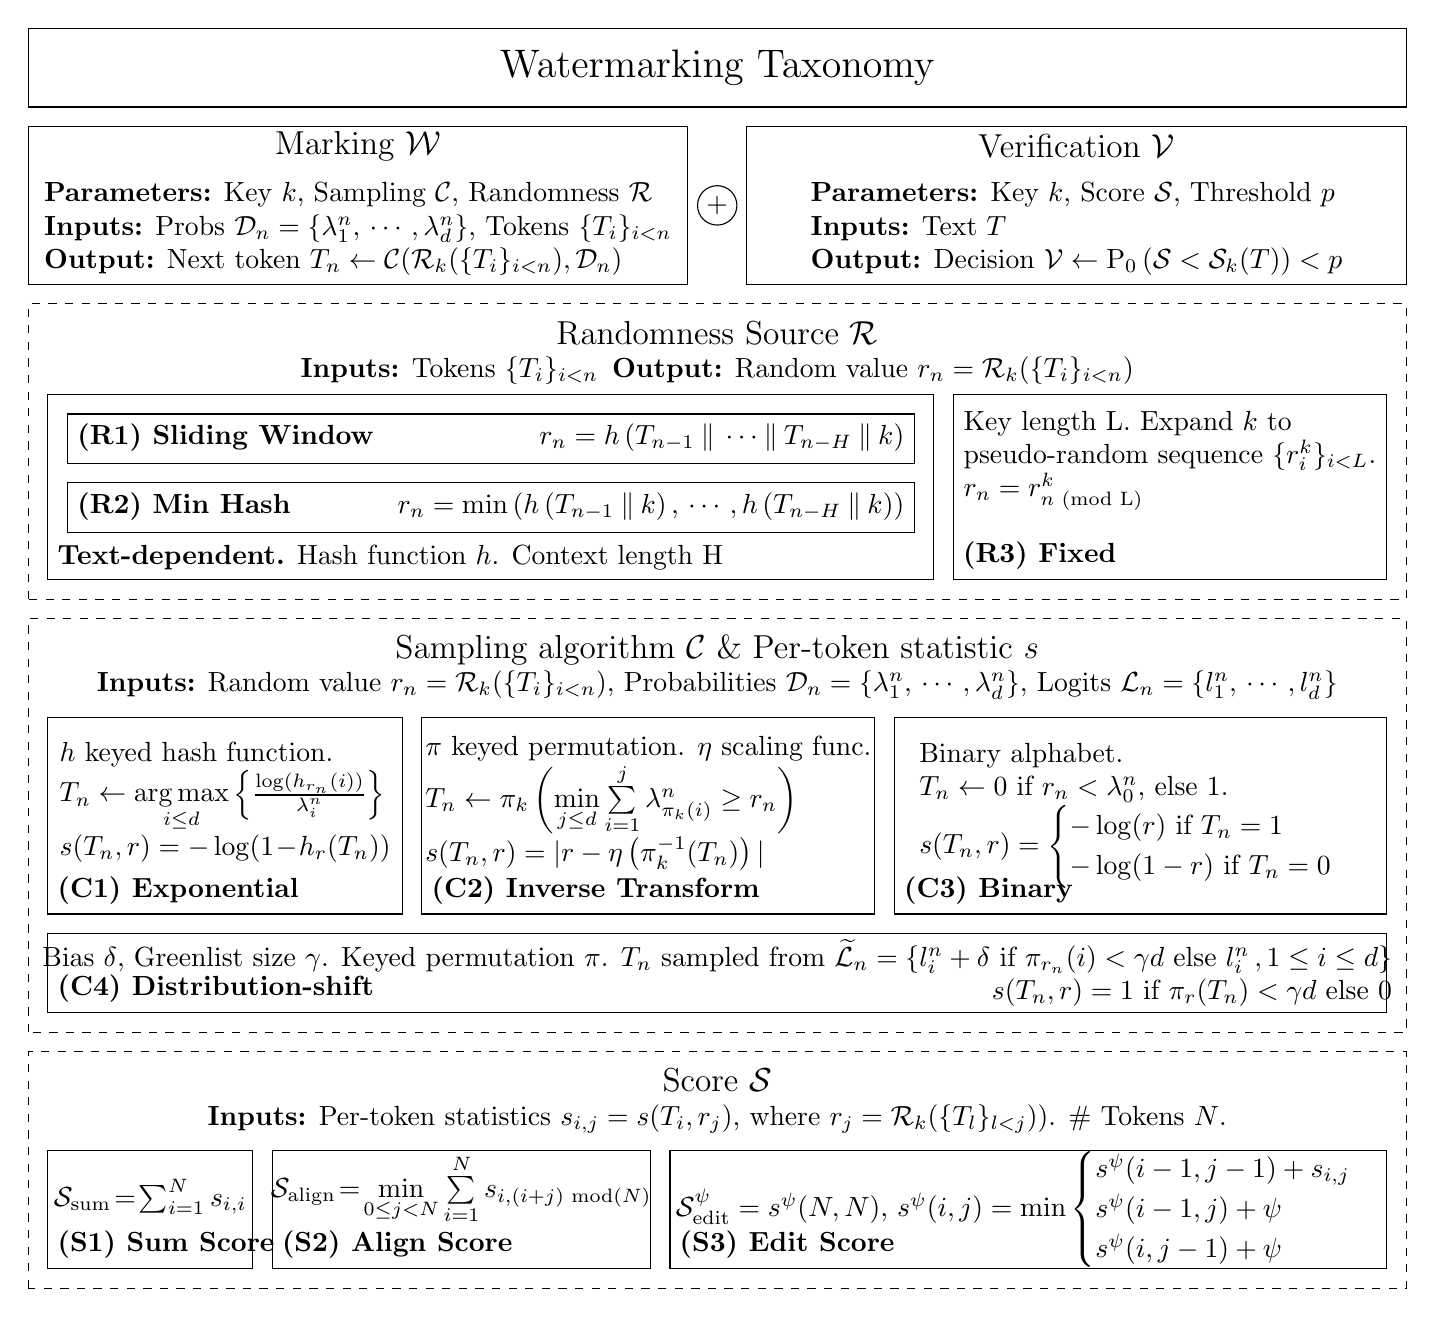
\begin{tikzpicture}
    
    \draw[draw=black] (0,15) rectangle ++(17.5,1) node[pos=0.5, align=center] {\Large{Watermarking Taxonomy}};
    \draw[draw=black] (0,12.75) rectangle ++(8.375,2) node[pos=0.5, align=left] 
    {\\
    \\
    \textbf{Parameters:} Key $k$, Sampling $\mathcal{C}$, Randomness $\mathcal{R}$\\
    \textbf{Inputs:} Probs $\mathcal{D}_n = \{\lambda^n_1,\, \cdots, \lambda^n_d\}$, Tokens $\{T_i\}_{i < n}$\\
    \textbf{Output:} Next token 
    $T_n \leftarrow \mathcal{C}(\mathcal{R}_k( \{T_i\}_{i < n}), \mathcal{D}_n)$};
    \draw[draw=black] (9.125,12.75) rectangle ++(8.375,2) node[pos=0.5, align=left] 
    {\\
    \\
    \textbf{Parameters:} Key $k$, Score $\mathcal{S}$, Threshold $p$\\
    \textbf{Inputs:} Text $T$\\
    \textbf{Output:} Decision $\mathcal{V} \leftarrow \text{P}_{0}\left( \mathcal{S} < \mathcal{S}_k(T)\right) < p$};
    \draw (8.75,13.75) circle (0.25) node {+};
    \draw[draw=none] (0,14.25) rectangle ++(8.375,.5) node[pos=0.5, align=left] {\large{Marking $\mathcal{W}$}};
    \draw[draw=none] (9.125,14.25) rectangle ++(8.375,.5) node[pos=0.5, align=left] {\large{Verification $\mathcal{V}$}};
    
    %%%
    
    \draw[draw=black,dashed] (0,8.75) rectangle ++(17.5,3.75);
    \draw[draw=none] (0,11) rectangle ++(17.5,1.75) node[pos=0.5, align=center] {\large{Randomness Source $\mathcal{R}$}\\
    \textbf{Inputs:} Tokens $\{T_i\}_{i < n}$\,
    \textbf{Output:} Random value $r_n = \mathcal{R}_k(\{T_i\}_{i < n})$};
    \draw[draw=black] (0.25,9) rectangle ++(11.25,2.35) node[pos=0, anchor=south west] {\textbf{Text-dependent.} Hash function $h$. Context length H};
    \draw[draw=black] (0.5,9.6) rectangle ++(10.75,0.625) node[anchor=north west] at (0.5, 10.225) {\textbf{(R2) Min Hash}} node[pos=1, anchor=north east, align=left] {
    $r_n = \text{min} \left( h\left( T_{n-1} \mathbin\Vert k\right), \, \cdots, h\left( T_{n-H} \mathbin\Vert k\right) \right)$\\
    };
    \draw[draw=black] (0.5,10.475) rectangle ++(10.75,0.625) node[anchor=north west] at (0.5, 11.1) {\textbf{(R1) Sliding Window}} node[pos=1, anchor=north east, align=left] {
    $r_n = h\left( T_{n-1} \mathbin\Vert \, \cdots \mathbin\Vert T_{n-H} \mathbin\Vert k\right)$\\
    };
    \draw[draw=black] (11.75,9) rectangle ++(5.5,2.35) node[pos=0, anchor=south west] {\textbf{(R3) Fixed}} node[pos=0.5, align=left] {Key length L. Expand $k$ to\\ pseudo-random sequence $\{r^k_i\}_{i<L}$.\\ 
    $r_n = r^k_{n \text{ (mod L)}}$ \\ \\ };
    
    %%%
    
    \draw[draw=black,dashed] (0,3.25) rectangle ++(17.5,5.25);
    \draw[draw=none] (0,6.85) rectangle ++(17.5,1.75) node[pos=0.5, align=center] {\large{Sampling algorithm $\mathcal{C}$ \& Per-token statistic $s$}\\
    \textbf{Inputs:} Random value $r_n = \mathcal{R}_k( \{T_i\}_{i < n})$, Probabilities $\mathcal{D}_n = \{\lambda^n_1,\, \cdots, \lambda^n_d\}$, Logits $\mathcal{L}_n = \{l^n_1,\,\cdots,l^n_d\}$\\};
    
    %
    
    \draw[draw=black] (11,4.75) rectangle ++(6.25,2.5) node[pos=0, anchor=south west] {\textbf{(C3) Binary}} node[pos=0.5, align=left] {Binary alphabet.\\ 
    $T_n \leftarrow 0$ if $r_n < \lambda^n_0$, else $1$. \\
    $s(T_n, r) = \begin{cases} -\log(r) \text{ if } T_n = 1\\
          -\log(1-r) \text{ if } T_n = 0\\\end{cases} $};
    
    \draw[draw=black] (5,4.75) rectangle ++(5.75,2.5) node[pos=0, anchor=south west] {\textbf{(C2) Inverse Transform}} node[pos=0.5, align=left] 
    {$\pi$ keyed permutation. $\eta$ scaling func.\\
    $T_n \leftarrow \pi_k \left( \min\limits_{ j \leq d } \sum\limits_{i=1}^j \lambda^n_{\pi_k (i)} \geq r_n \right)$ \\
    $s(T_n, r) = | r - \eta \left( \pi^{-1}_k(T_n) \right) | $\\};
    
    \draw[draw=black] (0.25,4.75) rectangle ++(4.5,2.5) node[pos=0, anchor=south west] {\textbf{(C1) Exponential}} node[pos=0.5, align=left] 
    {$h$ keyed hash function. \\
    $T_n \leftarrow \argmax\limits_{i \leq d} \left\{ \frac{\log \left( h_{r_n}\left( i \right) \right)}{\lambda^n_i} \right\}$ \\
    $s(T_n, r) = -\log(1 \! - \! h_r(T_n))$\\};
    
    % 
    
    \draw[draw=black] (0.25,3.5) rectangle ++(17,1) node[pos=0, anchor=south west] {\textbf{(C4) Distribution-shift}} node[pos=0.5, align=right] {Bias $\delta$, Greenlist size $\gamma$. Keyed permutation $\pi$. $T_n$ sampled from $\widetilde{\mathcal{L}}_n = \{l^n_i + \delta \text{ if } \pi_{r_n}(i) < \gamma d \text{ else } l^n_i\, , 1 \leq i \leq d\}$\\
    $s(T_n, r) = 1 \text{ if } \pi_{r}(T_n) < \gamma d \text{ else } 0$};
    
    %%% 
    
    \draw[draw=black,dashed] (0,0) rectangle ++(17.5,3);
    \draw[draw=none] (0,1.75) rectangle ++(17.5,1.25) node[pos=0.5, align=center] {\large{Score $\mathcal{S}$}\\
    \textbf{Inputs:} Per-token statistics $s_{i,j} = s(T_i, r_j)$, where $r_j = \mathcal{R}_k( \{T_l\}_{l < j}))$. \# Tokens $N$.};
    
    % 
    
    \draw[draw=black] (8.15,0.25) rectangle ++(9.1,1.5) node[pos=0, anchor=south west] {\textbf{(S3) Edit Score}}
    
    node[pos=0.5, align=left] {
    $\mathcal{S}_{\text{edit}}^\psi = s^\psi(N,N)$,
    $
        s^\psi (i,j) = \min \begin{cases}
          s^\psi (i-1, j-1) + s_{i,j}\\
          s^\psi (i-1, j) + \psi\\
          s^\psi (i, j-1) + \psi\\
        \end{cases} 
    $};
    \draw[draw=black] (0.25,0.25) rectangle ++(2.6,1.5) node[pos=0, anchor=south west] {\textbf{(S1) Sum Score}} node[pos=0.5, align=left] {$\mathcal{S}_{\text{sum}}\! = \! \sum_{i=1}^N s_{i,i}$ \\};
    \draw[draw=black] (3.1,0.25) rectangle ++(4.8,1.5) node[pos=0, anchor=south west] {\textbf{(S2) Align Score}} node[pos=0.5, align=left] {$\mathcal{S}_{\text{align}} \!= \!\min\limits_{0 \leq j < N} \sum\limits_{i=1}^N s_{i, (i+j) \text{ mod}(N)}$ \\ \\ };
    
    \end{tikzpicture}
    \caption{Watermarking design blocks. There are three main components: randomness source, sampling algorithm (and associated per-token statistics), and score function. Each solid box within each of these three components (dashed) denotes a design choice. The choice for each component is independent and offers different trade-offs.}\label{fig:design-figure}
    \end{center}
    \end{figure*}

\subsection{Watermark Design Space}
\label{sec:watermark-design}

Designing a good watermark is a balancing act.
% 
For instance, replacing every word of the output with [WATERMARK] would achieve high recall but destroy the utility of the model.
%
%Conversely, sampling from the original distribution preserves quality but makes it impossible to watermark. 

Existing proposals have cleverly crafted marking procedures that are meant to preserve quality, provide high precision and recall, and achieve a degree of robustness.
%
Despite their apparent differences, we realized they can all be expressed within a unified framework:

\begin{itemize}[leftmargin=\itemlm,itemsep=2pt]
    \item The marking procedure $\mathcal{W}$ contains a randomness source $\mathcal{R}$ and a sampling algorithm $\mathcal{C}$.
    %
    The randomness source $\mathcal{R}$ produces a (pseudo-random) value $r_n$ for each new token, based on the secret key $k$ and the previous tokens $T_0,\cdots,T_{n-1}$.
    %
    The sampling algorithm $\mathcal{C}$ uses $r_n$ and the model's next token distribution $\mathcal{D}$ to  a token.
    \item The verification procedure $\mathcal{V}$ is a one-tailed significance test that computes a $p$-value for the null hypothesis that the text is not watermarked.
    %
    The procedure compares this $p$-value to a threshold, which enables control over the watermark's precision and recall.
    %
    % This test is done using a \emph{score function} $\mathcal{S}$ based on a per-token variable that depends on the ed sampling algorithm.
    % We call the value of this per-token test statistic $s_n$, which only depends on the random value $r_n$ and the ed token $T_n$: $s_n = s(T_n, r_n)$.
    In particular, we compute a per-token score $s_{n,m} \coloneqq s(T_n, r_m)$ for each token $T_n$ and randomness $r_m$, aggregate them to obtain an overall score $\mathcal{S}$, and compute a $p$-value from this score.
    We consider all overlaps $s_{n,m}$ instead of only $s_{n,n}$ to support scores that consider misaligned randomness and text after perturbation. 
    %the test computes \emph{score function} $\mathcal{S}$ which takes as input per-token test statistics $s_{n,m} \coloneqq s(T_n, r_m)$ for a token $T_n$ and a random value $r_m$, $\forall n,m \in [N]$.
    %
    %$s_{n,m}$ depends on the sampling algorithm (see \cref{fig:design-figure} for examples).
    %
    % \dave{I believe $s(T_n, r_m)$ is incorrect and it should be $s(T_n, r_n)$.  Also I think the score should be $s_n$ rather than $s_{n,m}$.}
    % \jp{Depending on the alignment between the key string and the text, there are times we want to refer to the score for key at position m and token at poistion n (for instance, for both the align and edit scores). I'll add some explanation for this.}
    
\end{itemize}
% \dave{I find the sheer number of fonts inelegant (blackboard bold, mathcal, mathbf, typewritter, italics, bold, etc.). In some places, algorithms are denoted by mathcal (W,V), in other places by mathbf (R,C,S).  I suggest picking one and being consistent.  I prefer mathcal.  Lots of bold feels distracting to my eyes, as does lots of font changes.}
% \jp{I changed a bunch of fonts to make it more consistent, and removed bold fonts}

Next, we show how each scheme we consider falls within this framework, each with its own choices for $\mathcal{R},\mathcal{C},\mathcal{S}$.
%Given this template, previous work introduced their own variants of the building blocks, which we will now detail. 
% \chawin{I would have liked to see a summary of which design choices belong to which paper. Maybe we can add a shorthand notation denoting each paper in \cref{fig:design-figure} or have a separate table.}
% \jp{I agree that's a good idea. A table is probably the right way to represent this.}

\subsubsection{Randomness source $\mathcal{R}$}\label{ssec:randomness}
% \textbf{Randomness source $\mathcal{R}$.}
%
% \chawin{Maybe others?} \jp{Yeah but all the other papers i've seen seem to attribute it to one of these two.}
We distinguish two main ways of generating the random values $r_n$, \emph{text-dependent} (computed as a deterministic function of the prior tokens) vs \emph{fixed} (computed as a function of the token index).
Both approaches use the standard heuristic of applying a keyed function (typically, a PRF) to some data, to produce pseudorandom values that can be treated as effectively random but can also be reproduced by the verification procedure.

\citet{aaronson_watermarking_2022} and \citet{kirchenbauer_watermark_2023}
use text-dependent randomness: $r_n = f\left(T_0,\,\cdots,T_{n-1},k\right)$.
%
This scheme has two parameters: the length of the token context window (which we call the window size H) and the aggregation function $f$.
%
\citet{aaronson_watermarking_2022} proposed using the hash of the concatenation of previous tokens, $f := h\left( T_{n-1} \mathbin\Vert \, \cdots \mathbin\Vert T_{n-H} \mathbin\Vert k\right)$; we call this (R1) sliding window.
%
\citet{kirchenbauer_watermark_2023} used this with a window size of $ H = 1$ and also introduced an alternate aggregation function $f := \text{min} \left( h\left( T_{n-1} \mathbin\Vert k\right), \, \cdots, h\left( T_{n-H} \mathbin\Vert k\right) \right)$.
%
We call this last aggregation function (R2) min hash.
%
While these two schemes propose specific choices of $H$, other values are possible. 
We use \benchmarkname{} to evaluate a range of values of $H$ with each candidate aggregation function.

% \smallskip\noindent\textbf{(R3) Fixed}
\citet{kuditipudi_robust_2023} use fixed randomness:
$r_n = f_k(n)$, where $n$ is the index (position) of the token.
We call this (R3) fixed.
%
In practice, they propose using a fixed string of length $L$ (the key length), which is repeated across the generation.
% r_n = f_k(n \bmod L)$ where $L$ is the key length.
% \dave{I don't think we need this level of detail.  I suggest deleting the preceding sentence.}
% \jp{Since we look at the impact of the key length on generations we still need to introduce the idea that the key is repeated, but I canwrite that in english for it to be more digestable}
%
We test the choice of key length in ~\cref{ssec:param_tuning}
%
In the extreme case where $L=1$ or $H=0$, both sources are identical, as $r_n$ will be the same value for every token. \citet{zhao2023provable} explored this option using the same sampling algorithm as~\citet{kirchenbauer_watermark_2023}.

\label{ssec:binary}
\citet{christ_undetectable_2023} proposed setting a target entropy for the context window instead of fixing a window size.
%
This allows to set a lower bound on the security parameter for the model's undetectability.
%
However, setting a fixed entropy makes for a less efficient detector since all context window lengths must be tried in order to detect a watermark.
%
Furthermore, in practice, provable undetectability is not needed to achieve optimal quality: we chose to keep using a fixed-size window for increased efficiency.

\subsubsection{Sampling algorithm \(\mathcal{C}\)}\label{ssec:sampling}
% \textbf{sampling algorithm $\mathcal{C}$.}
%
\noindent
We now give more details about the four sampling algorithms initially presented in~\cref{tab:marking-algorithms}.

\smallskip\noindent\textbf{(C1) Exponential}.
%
Introduced by \citet{aaronson_watermarking_2022} and also used by \citet{kuditipudi_robust_2023}. It relies on the Gumbel-max trick.
%
Let $\mathcal{D}_n = \left\{\lambda^n_i\,, 1 \leq i \leq d\right\}$ be the distribution of the language model over the next token. %(obtained after passing the logits through a softmax and applying a temperature adjustment).
%
The exponential scheme will select the next token as:
\begin{align}
    T_{n} = \argmax\limits_{i \leq d}\left\{ \frac{\log \left( h_{r_n}\left( i \right) \right)}{\lambda^n_i} \right\}
\end{align}
where $h$ is a keyed hash function using $r_n$ as its key.
%
The per-token variable used in the statistical test is either $s_n = h_{r_n}(T_n)$ or $s_n = -\log \left( 1-h_{r_n}(T_n)\right)$.
%
\citet{aaronson_watermarking_2022} and \citet{kuditipudi_robust_2023} both use the latter quantity.
%
We argue the first variable provides the same results, and unlike the log-based variable, the distribution of watermarked variables can be expressed analytically (see~\cref{app:ssec:pseudorandom-proofs} for more details).
%
We align with previous work and use the $\log$ for \benchmarkname{}.

\smallskip\noindent\textbf{(C2) Inverse transform}.
%
\citet{kuditipudi_robust_2023} introduce inverse transform sampling.
%
They derive a random permutation using the secret key $\pi_k$. The next token is selected as follows:
\begin{align}
    T_{n} = \pi_k \left( \min\limits_{ j \leq d } \sum\limits_{i=1}^j \lambda^n_{\pi_k (i)} \geq r_n \right)
\end{align}
which is the smallest index in the inverse permutation such that the CDF of the next token distribution is at least $r_n$.
%
\citet{kuditipudi_robust_2023} propose to use $s_n = | r_n - \eta \left( \pi^{-1}_k(T_n) \right) |$ as a the test variable, where $\eta$ normalizes the token index to the $[0,1]$ range.
%
% We call this scheme the \textit{inverse transform} scheme.

\smallskip\noindent\textbf{(C3) Binary}.
%
\citet{christ_undetectable_2023} propose a different sampling scheme for binary token alphabets --- however, it can be applied to any model by using a bit encoding of the tokens.
%
In our implementation, we rely on a Huffman encoding of the token set, using frequencies derived from a large corpus of natural text.
%
In this case, the distribution over the next token reduces to a single probability $p_n$ that token ``0'' is ed next, and $1-p$ that ``1'' is ed.
%
The sampling rule s 0 if $r_n < p$, and 1 otherwise. The test variable for this case is $s_n = -\log \left( T_n r_n + (1-T_n) (1-r_n) \right)$.
%
% We call this scheme the \textit{binary} scheme.
%
% At first glance, it can seem like this scheme is identical to the exponential scheme. However, because it uses a binary alphabet, the distribution of the test variable is different for both schemes.
%
% However, we show in Appendix \jp{ref} that this is not the case: the distribution of the test variable is different for both schemes.
% %
% \jp{Maybe I'll remove this if I don't have time to show it.}

\smallskip\noindent\textbf{(C4) Distribution-shift}.
%
\citet{kirchenbauer_watermark_2023} propose the distribution-shift scheme. 
%
It produces a modified distribution $D_n$ from which the next token is sampled.
%
Let $\delta > 0$ and $\gamma \in [0,1]$ be two system parameters, and $d$ be the number of tokens.
%
The scheme constructs a permutation $\pi_{r_n}$, seeded by the random value $r_n$, which is used to define a ``green list,'' containing tokens $T$ such that $\pi_{r_n} (T) < \delta d$. It then adds $\delta$ to green-list logits.
%
This modified distribution is then used by the model to sample the next token. The test variable $s_n$ is a bit equal to ``1'' if $T_n$ is in the green list defined by $\pi_{r_n}$, and ``0'' if not.
%
% We call this scheme the \textit{distribution-shift} scheme.

The advantage of this last scheme over the others is that it preserves the model's diversity: 
for a given key, the model will still generate diverse outputs.
In contrast, for a given secret key and a given prompt, the first three sampling strategies 
will always produce the same result, since the randomness value $r_n$ will be the same.
\citet{kuditipudi_robust_2023} tackles this by randomly offseting the key sequence of 
fixed randomness for each generation. We introcude a skip probability $p$ for the 
same effect on text-dependent randomness. Each token is selected without the marking 
strategy with probability $p$. In the interest of space, we leave a detailed discussion 
of generation diversity in~\cref{app:ssec:diverse}.

Another advantage of the distribution-shift scheme is that it can also be used 
at any temperature, by applying the temperature scaling \emph{after} using the 
scheme to modify the logits. Other models apply temperature before watermarking.

However the distribution-shift scheme is not indistinguishable from the original model, 
as discussed earlier in~\cref{ssec:watermark-design}.

\subsubsection{Score Function $\mathcal{S}$}\label{ssec:score}

% \paragraph{Verification procedure $\mathcal{V}.$}

% The distribution of the per-token test statistic is different for watermarked text and non-watermarked text: this is what makes detection possible. Depending on the scheme, it is either higher or lower on average in the watermarked case. Without loss of generality, we assume it is always lower for this discussion.

To determine whether an $N$-token text is watermarked, we compute a score over per-token statistics.
%
This score is then subject to a one-tailed statistical test where the null hypothesis is that the text is not watermarked.
%
In other words, if its $p$-value is under a fixed threshold, the text is watermarked.
%
Different works propose different scores.

\smallskip\noindent\textbf{(S1) Sum score}.
%
\citet{aaronson_watermarking_2022} and \citet{kirchenbauer_watermark_2023} take the sum of all individual per-token statistics:
\begin{align}
    \mathcal{S}_{\text{sum}}=\sum_{i=1}^N s_i = \sum_{i=1}^N s(T_i, r_i).
\end{align}
%
This score requires the random values $r_i$ and the tokens $T_i$ to be aligned.
%
% \chawin{Maybe this goes into limitation or discussion or appendix}
This is not a problem when using text-dependent randomness, since the random values are directly obtained from the tokens.
%
However, this score is not suited for fixed randomness: removing one token at the start of the text will offset the values of $r_i$ for the rest of the text and remove the watermark.
%
The use of the randomness shift to increase diversity will have the same effect. 

\smallskip\noindent\textbf{(S2) Alignment score}.
Proposed by \citet{kuditipudi_robust_2023}, the alignment score aims to mitigate the misalignment issue mentioned earlier.
% \citet{kuditipudi_robust_2023} proposes two alternative scores to deal with this issue.
%
% In keeping with their work, we name these scores the alignment score and the edit score.
Given the sequence of random values $r_i$ and the sequence of tokens $T_i$, the verification process now computes different versions of the per-token test statistic for each possible overlap of both sequences $s_{i,j} = s(T_i, r_j)$.
%
The alignment score is defined as:
\begin{align}
   \mathcal{S}_{\text{align}}  = \min\limits_{0 \leq j < N} \sum\limits_{i=1}^N s_{i, (i+j) \text{ mod}(N)}
\end{align}

\smallskip\noindent\textbf{(S3) Edit score}.
Similar to the alignment score, \citet{kuditipudi_robust_2023} propose the edit score as an alternative for dealing with the misalignment issue.
%
It comes with an additional parameter $\psi$ and is defined as $\mathcal{S}_{\text{edit}}^\psi = s^\psi(N,N)$, where
\begin{align}
    s^\psi (i,j) &= \min \begin{cases}
      s^\psi (i-1, j-1) + s_{i,j}\\
      s^\psi (i-1, j) + \psi\\
      s^\psi (i, j-1) + \psi\\
    \end{cases} 
\end{align}

In all three cases, the average value of the score for watermarked text will be lower than for non-watermarked text.
%
% In the case of the sum score, we can often derive the distribution of the score under the null hypothesis, allowing us to use a $z$-test to determine if the text is watermarked.
In the case of the sum score, the previous works use the $z$-test on the score to determine whether the text is watermarked, but it is also possible, or even better in certain situations, to use a different statistical test according to \citet{fernandez_three_2023}.
%
When possible, we derive the exact distribution of the scores under the null hypothesis (see \cref{app:ssec:exact_dist}) which is more precise than the $z$-test. When it is not, we rely on an empirical T-test, as proposed by \citet{kuditipudi_robust_2023}
%
% This allows one to compute 

\subsection{Limitations of the Building Blocks}\label{ssec:limit_blocks}

While we design the blocks to be as independent as possible, some combinations of the scheme and specific parameters are obviously sub-optimal.
%
Here, we list a few of these subpar block combinations as a guide for practitioners.
% Even though any of the three scores can be used with any scheme and randomness source, in practice not all combinations are useful.
\begin{itemize}[leftmargin=\itemlm,itemsep=2pt]
    \item The sum score (S1) is not robust for fixed randomness (R3).
    \item The alignment score (S2) does not make sense for the text-dependent randomness (R1, R2) since misalignment is not an issue.
    \item The edit score (S3) has a robustness benefit since it can support local misalignment caused by token insertion, deletion, or swapping. However, using it with text-dependent randomness (R1, R2) only makes sense for a window size of 1: for longer window sizes, swapping, adding, or removing tokens would actually change the random values themselves, and not just misalign them.
    \item Finally, in the corner case when a window size of 0 for the text-dependent randomness (R1, R2) or when a random sequence length of 1 for the fixed randomness (R3), both the alignment score (S2) and the edit score (S3) are unnecessary since all random values are the same and misalignment is not possible.
\end{itemize}

In our experiments (\cref{sec:experiments}), we test all reasonable configurations of the randomness source, 
the sampling protocol, and the verification score, along with their parameters. 
We list the evaluated combinations in~\cref{tab:design_space_combinations}. 
The edit score is too inefficient 
to be run on all configurations, instead we rely on the sum and align scores.
%
We hope to not only fairly compare the prior works but also investigate previously unexplored combinations in the 
design space that can produce a better result.

% \chawin{We need a table or a tree that lists all the combinations we test.}\

\begin{table}[h!]
    \centering
    \caption{Tested combinations in the design space, using notations from~\cref{fig:design-figure}.\\
    We only tested the edit score {\bf S3} on a subset of watermarks.\\
    The distribution of non-watermarked scores is known for \textcolor{orange}{orange} configurations and 
    unknown for \textcolor{blue}{blue} configuration. We rely on empirical T-tests~\cite{kuditipudi_robust_2023} for blue configurations.
    }
    \label{tab:design_space_combinations}
    \normalsize
    \begin{tabular}{|l||c|c|c|c|} 
    \hline
     & \makecell[tc]{{\bf C4}\\{\small Distribution}\\{\small Shift}} & \makecell[tc]{{\bf C1}\\{\small Exponential}} & \makecell[tc]{{\bf C2}\\{\small Binary}} & \makecell[tc]{{\bf C3}\\{\small Inverse}\\{\small Transform}} \\
    \hline
    \hline
    \makecell{{\bf S1}+{\bf R1}}  & \textcolor{orange}{X} & \textcolor{orange}{X} & \textcolor{orange}{X} & \textcolor{blue}{X} \\
    \hline
    \makecell{{\bf S1}+{\bf R2}}  & \textcolor{orange}{X} & \textcolor{orange}{X} & \textcolor{orange}{X} & \textcolor{blue}{X} \\
    \hline
    \makecell{{\bf S2}+{\bf R3}}  & \textcolor{blue}{X} & \textcolor{blue}{X} & \textcolor{blue}{X} & \textcolor{blue}{X} \\
    \hline
    \makecell{{\bf S3}+{\bf R3}}  & \textcolor{blue}{X} &  &  &  \\
    \hline
    \end{tabular}
\end{table}
    

\subsection{Analysis of the edit score.} 
\label{ssec:editscore}
We analyzed the tamper-resistance of the edit score on a subset of watermarks 
(distribution-shift with $\delta=2.5$ at a temperature of 1, for key lengths between 1 and 1024). 
We tried various $\psi$ values between 0 and 1 for the edit distance, and compared the tamper-resistance 
and watermark size of the resulting verification procedures to the align score. 
Using an edit distance does improve tamper-resistance for key lengths under 32, but at a large efficiency cost: 
for key lengths above 8, the edit score size is at least twice that of the align score. 
We do not recommend using an edit score on low entropy models such as Llama-2 chat.





\section{Summary}

We performed a series of galactic disk $N$-body simulations
to investigate the formation and dynamical evolution of spiral arm 
and bar structures in stellar disks which are embedded in live 
dark matter halos.
We adopted a range of initial conditions where the models have similar halo 
rotation curves, but different masses for the disk and bulge components, 
scale lengths, initial $Q$ values, and halo spin parameters.
The results indicate that the bar formation epoch increases exponentially 
as a function of the disk mass fraction with respect to the total mass at the 
reference radius (2.2 times the disk scale length), $f_{\rm d}$.
This relation is a consequence of swing amplification~\citep{1981seng.proc..111T},
which describes the amplification rate of the spiral arm when it transitions from 
leading arm to trailing arm because of the disk's differential rotation.
Swing amplification depends on the properties that characterize the disk, 
Toomre's $Q$, $X$, and $\Gamma$. The growth rate reaches its maximum
for $1<X<2$,  although the position of the peak slightly depends on $Q$ as well as on
$\Gamma$. We computed $X$ for 
$m=2$ ($X_2$), which corresponds to a bar or two-armed spiral, 
for each of our models and found that this value is related to the bar's
formation epoch.

The bar amplitude grows most efficiently when $1<X_2<2$. For models 
with $1<X_2<2$ the bar develops immediately after the start 
of the simulation. As $X_2$ increases beyond $X_2=2$, the growth rate
decreases exponentially. We find that the bar formation epoch increases
exponentially as $X_2$ increases beyond $X_2=2$, in other words
$f_{\rm d}$ decreases. The bar formation epoch exceeds a Hubble time
for $f_{\rm d}\lesssim 0.35$.

Apart from $X$, the growth rate is also influenced by $Q$ where
a larger $Q$ results in a slower growth. This indicates that the bar formation
occurs later for larger values of $Q$. 
Our simulations confirmed this and showed that for the bar ($m=2$) the growth rate
is predicted by swing amplification and becomes visible when it grows beyond a certain amplitude.

Toomre's swing amplification theory further predicts that
the number of spiral arms is related to the mass of the disk, with
massive disks having fewer spiral arms. In addition, larger $\Gamma$
predicts a smaller number of spiral arms.
We confirmed these relations in our simulations. 
The shear rate ($\Gamma$) also affects the pitch angle of spiral
  arms. We further confirmed that our result is consistent with previous
studies.

We found that the disk-to-total mass fraction ($f_{\rm d}$)
and the shear rate ($\Gamma$) are the most important parameters that determine the
morphology of disk galaxies. 
When juxtaposing our models with the Hubble sequence,
the fundamental subdivisions of (barred-)spiral galaxies with 
massive bulges and tightly wound-up spiral arms from S(B)a to S(B)c is 
also be observed as a sequence in our simulations. Where the models 
with either massive bulges or massive disks have more tightly
wound spiral arms. This is because having both a massive disk and bulge results in 
a larger $\Gamma$, i.e., more tightly wound spiral arms. 


Once the
bar is formed it starts to heat the outer parts of the disk.
From this point onwards, 
the self-gravitating spiral arms disappear.
This may be in part caused by the 
lack of gas in our simulations. 
After the bar grows, we no longer discern  
spiral arms in the outer regions of the disk. This could imply
that gas cooling and star formation are required in order to 
maintain spiral structures in barred spiral galaxies for over 
a Hubble time~\citep{1981ApJ...247...77S,1984ApJ...282...61S}.


Our simulations further indicate that non-barred grand-design spirals are
transient structures which immediately evolve into barred
galaxies. Swing amplification teaches us that a massive disk is
required to form two-armed spiral galaxies. This condition, at the
same time, satisfies the short formation time of the bar structure.
Non-barred grand-design spiral galaxies therefore must evolve into barred
galaxies.  We consider that isolated non-barred grand-design spiral galaxies 
are in the process of developing a bar.




\bibliography{refs}
% \bibliographystyle{abbrvnat}
\bibliographystyle{IEEEtranN}
\newpage

\appendix
% \section{Detailed Description of Watermark Design Space}\label{app:sec:watermark}

\subsection{Techniques to Allow Diverse Generation}\label{app:ssec:diverse}

In order to add some diversity to the generations, there are different strategies.
\begin{enumerate}[leftmargin=\itemlm,itemsep=2pt]
    \item For a fixed randomness source, \citet{kuditipudi_robust_2023} proposes to randomly shift the sequence of random values $\{r^k_i\}$ by an offset $s$, such that $r_n = r^k_{(s+n) \text{ (mod L)}}$. This means there are a total of $L$ possible unique values for $r_n$ depending on $s$. For a text-dependent randomness source, this trick does not work. 
    \item Instead, one natural strategy is to randomly skip the watermarking selection procedure for some tokens, and instead sample the next token from the original multinomial distribution. We denote \textbf{S} this skip probability. 
    \item Another strategy, discussed by \citet{christ_undetectable_2023}, is to only start watermarking text after enough empirical entropy has been generated: the first tokens are selected without a watermark. This accomplishes the same effect, and guarantees undetectability. However, as discussed in the paper's appendix, a user not wanting to generate watermarked text can simply run the model, keep the first few tokens, add them to the prompt, and start again: After repeating this step enough time, they can generate arbitrarily long text without a watermark. This seems like a larger practical drawback than loosing the guarantee of undetectability, thus we use the skip probability instead for promoting diversity. 
\end{enumerate}

\subsection{Exact Distribution of the Score Function}\label{app:ssec:exact_dist}

The null hypothesis distribution for the exponential scheme with the regular test variable is an Irwin-Hall distribution centered with parameter $N$ (whose average quickly converges to a normal distribution centered in 0.5 with variance $\frac{1}{12N}$).
%
When using the log test variable, the null distribution is the Erlang distribution with parameter $N$. The binary scheme also follows an Erlang distribution, but with many more tokens since each token is broken down into a binary vector. The distribution-shift scheme has a null distribution a binomial with parameters $\gamma, N$. We derive these distributions in the appendix.

However, for both other scores, and for the inverse transform, the null hypothesis distribution is too complex to compute. In these cases, verification uses a permutation test, as described in Kuditipudi et al.. Instead of comparing the score to a known distribution, we sample independent random sequences $\tilde{r}_i$ and compute the score of the text for that randomness: these trials are distributed like non watermarked text, so we can use them to compute an empirical p-value. 
\subsection{Additional analysis}
\label{app:ssec:additional_figures}

Here we present additional figures to support the main text.

\begin{figure}
    \centering
    \includegraphics[width=1\linewidth]{figures/fig1b.png}
    \caption{Same plot as~\cref{fig:aggregate}, but for a quality threshold of 10\%, and a minimum robustness of 0.2. The same conclusions from the main figure still hold.}
    \label{fig:aggregate2}
\end{figure}

\begin{figure}[t]
    \includegraphics[width=\linewidth]{figures/robustness_to_attack.png}
    \centering
    \caption{Correlation between robustness metric and attack success. On the right, for the Russian translation attack. 
    On the left, for the GPT paraphrasing attack. Each dot is a unique watermark parameter setting.}
    \label{fig:robustness-to-attacks}
\end{figure}

\begin{figure}[t]
\includegraphics[width=\linewidth]{figures/delta.png}
\centering
\caption{Size and quality for varying biases, at T=0.3 and T=1. The quality is relative to the quality of the non-watermarked model at the given temperature.}
\label{bias-fig}
\end{figure}

\begin{figure}[t]
\includegraphics[width=\linewidth]{figures/keylen.png}
\centering
\caption{Size and tamper resistance as a function of key lengths (only using distribution-shift schemes with $\delta \leq 2$).}
\label{keylen-fig}
\end{figure}
\section{Proofs from \secref{sec:qkd}}
\label{app:proofs}

In \secref{sec:qkd} we show how to define the security of QKD in a
composable framework and relate this to the trace distance security
criterion introduced in \textcite{Ren05}. This composable treatment of
the security of QKD follows the literature \cite{BHLMO05,MR09}, and
the results presented in \secref{sec:qkd} may be found in
\textcite{BHLMO05,MR09} as well. The formulation of the statements
differs however from those works, since we use here the Abstract
Cryptography framework of \textcite{MR11}. So for completeness, we
provide here proofs of the main results from \secref{sec:qkd}.

\begin{proof}[Proof of \thmref{thm:qkd}]
  Recall that in \secref{sec:security.simulator} we fixed the
  simulator and show that to satisfy \eqnref{eq:qkd.security} it is
  sufficient for \eqnref{eq:qkd.security.2} to hold. Here, we will
  break \eqnref{eq:qkd.security.2} into security [\eqnref{eq:qkd.cor}]
  and correctness [\eqnref{eq:qkd.sec}], thus proving the theorem.

  Let us define $\gamma_{ABE}$ to be a state obtained from
  $\rho^{\top}_{ABE}$ [\eqnref{eq:qkd.security.tmp}] by throwing away
  the $B$ system and replacing it with a copy of $A$, i.e., \[
  \gamma_{ABE} = \frac{1}{1-p^\bot} \sum_{k_A,k_B \in \cK} p_{k_A,k_B}
  \proj{k_A,k_A} \otimes \rho^{k_A,k_B}_E.\] From the triangle
  inequality we get \begin{multline*} D(\rho^\top_{ABE},\tau_{AB} \otimes
  \rho^\top_{E}) \leq \\ D(\rho^\top_{ABE},\gamma_{ABE}) +
  D(\gamma_{ABE},\tau_{AB} \otimes \rho^\top_{E}) .\end{multline*}

Since in the states $\gamma_{ABE}$ and
$\tau_{AB} \otimes \rho^\top_{E}$ the $B$ system is a copy of the $A$
system, it does not modify the distance. Furthermore,
$\trace[B]{\gamma_{ABE}} =
\trace[B]{\rho^{\top}_{ABE}}$. Hence
\[D(\gamma_{ABE},\tau_{AB} \otimes \rho^\top_{E}) =
  D(\gamma_{AE},\tau_{A} \otimes \rho^\top_{E}) =
  D(\rho^\top_{AE},\tau_{A} \otimes \rho^\top_{E}).\]

For the other term note that
\begin{align*}
  & D(\rho^\top_{ABE},\gamma_{ABE}) \\
  & \qquad \leq \sum_{k_A,k_B} \frac{p_{k_A,k_B}}{1-p^{\bot}}
    D\left(\proj{k_A,k_B} \otimes \rho^{k_A,k_B}_E,\right. \\
  & \qquad \qquad \qquad \qquad \qquad \qquad \left.\proj{k_A,k_A} \otimes \rho^{k_A,k_B}_E \right)\\
  & \qquad = \sum_{k_A \neq k_B} \frac{p_{k_A,k_B}}{1-p^{\bot}} = \frac{1}{1-p^{\bot}}\Pr
  \left[ K_A \neq K_B \right].
\end{align*}
Putting the above together with \eqnref{eq:qkd.security.2}, we get
\begin{align*} & D(\rho_{ABE},\tilde{\rho}_{ABE}) \\
  & \qquad = (1-p^\bot)
  D(\rho^\top_{ABE},\tau_{AB} \otimes \rho^\bot_{E}) \\ & \qquad \leq \Pr
  \left[ K_A \neq K_B \right] + (1-p^\bot) D(\rho^\top_{AE},\tau_{A}
  \otimes \rho^\top_{E}). \qedhere \end{align*}
\end{proof}

\begin{proof}[Proof of \lemref{lem:robustness}]
  By construction, $\aK_\delta$ aborts with exactly the same
  probability as the real system. And because $\sigma^{\qkd}_E$
  simulates the real protocols, if we plug a converter $\pi_E$ in
  $\aK\sigma^{\qkd}_E$ which emulates the noisy channel $\aQ_q$ and
  blogs the output of the simulated authentic channel, then
  $\aK_\delta = \aK\sigma^{\qkd}_E\pi_E$. Also note that by
  construction we have
  $\aQ_q \| \aA' = \left(\aQ \| \aA\right) \pi_E$. Thus
  \begin{multline*} d\left( \pi_A^{\qkd}\pi_B^{\qkd}(\aQ_q \| \aA')
      ,\aK_\delta\right) \\ = d\left( \pi_A^{\qkd}\pi_B^{\qkd}\left(\aQ
        \| \aA\right) \pi_E , \aK\sigma^{\qkd}_E\pi_E\right). \end{multline*}

  Finally, because the converter $\pi_E$ on both the real and ideal
  systems can only decrease their distance (see
  \secref{sec:ac.systems}), the result follows.
\end{proof}


%%% Local Variables:
%%% TeX-master: "main.tex"
%%% End:


\end{document}
